\documentclass[a4paper,11pt]{article}
\usepackage[utf8]{inputenc}
\usepackage[T1]{fontenc}
\usepackage[french]{babel}
\usepackage{makeidx}
\usepackage{textcomp}
\usepackage{graphicx}
\usepackage{mathtools,amssymb,amsthm}
\usepackage{lmodern}
\usepackage{multirow}
\usepackage{listings}
\usepackage{array}
\usepackage{hyperref}
\usepackage{longtable}

\title{Projet simulation - Rapport}
\author{Maxime Gonthier (21500231) - Benjamin Guillot (21500545)}

\begin{document}
\pagenumbering{gobble}\clearpage
\maketitle

\newpage
\tableofcontents

\newpage
\section{Introduction}
	L'objectif de ce projet est de simuler en temps discret des arrivées et des services dans un cyber café. On en déduira des mesures d'évaluations à l'aide du calcul du temps moyen d'attente et du $90_{ème}$ percentile du temps d'attente.\\
	A l'issu de ce projet, on sera capable de dire parmi 3 modèle le ou lesquels sont plus adapté au service dans le cyber café.
\newpage
\section{Explication de la programmation}
	\subsection{Entrée et sortie du programme}
	En entrée le programme prend un fichier texte contenant les données que l'on veut faire varier dans notre application (ici lambda).
	On obtient en sortie 2 fichier :
	\begin{itemize}
		\item resultE.txt
		\item result90.txt
	\end{itemize}
	Ces deux fichiers contiennent respectivement les temps d'attente moyen pour chaque modèles en fonction de lambda et les 90 percentile du temps d'attente de chaque modèles, également en fonction de lambda.\\
	Ils sont utiliser pour tracer les courbes que l'on pourra observer dans la section \hyperref[Analyse des résultats]{Analyse des résultats}
	\subsection{structure du programme}
	Nous avons choisit pour la programmation de gérés les différents modèles dans les fonctions $Arrivee\_Client$ et $service\_event$. Ces deux fonctions on 3 modes de fonctionnement
	passé en argument pour savoir quel modèle on est en train de simuler. Il y a un simulateur par modèles.
	Il sont appelés dans le main avec en argument :
	\begin{itemize}
		\item un fichier dans lequel écrire les données relatives a la simulation.
		\item la valeur de lambda en train d'être testée.
	\end{itemize}
	Détails en \hyperref[annexe]{annexe}
	\subsubsection{premier modèle}
		le premier modèle représente une M/M/N classique. on traite donc les clients dès qu'un serveur est libre.
	\subsubsection{second modèle}
		Le second modèle peut être simulé avec une M/M/1. On ajoute une condition aux arrivées de client qui est un pourcentage de chance d'arriver dans la file, comme on a 10 serveurs en théorie, un client arrive dans une file avec une probabilité $\frac{1}{10}$.
	\subsubsection{troisième modèle}
		Le troisième modèle est simulé avec 10 M/M/1. On stocke dans un tableau le nombre de client par file et a chaque arrivée de client, on vérifie quelle est la file la moins remplie. Le client est envoyé sur cette file. On stocke dans l'évènement la file sur laquelle se trouve le client afin de pouvoir décrémenter le nombre de client de cette file après un service. 
	
\section{Analyse des résultats}
\label{Analyse des résultats}
	Avant tout de chose, notons que pour le modèle 2, les valeurs que nous avons obtenus pour le temps moyen d'attente
	correspondent à 1/10 des clients d'une M/M/1. Ce qui revient au final à créer 10 M/M/1. Nous avons choisis cette ordre de grandeur
	plus petit pour pouvoir dessiner les 3 courbes sur le même graphe sans avoir à déformer énormément l'echelle. En effet sinon nous aurions dû 
	multiplier par 10 toutes les valeurs du temps moyen d'attente pour le modèle 2.\\
	\label{fig1}
	\centerline{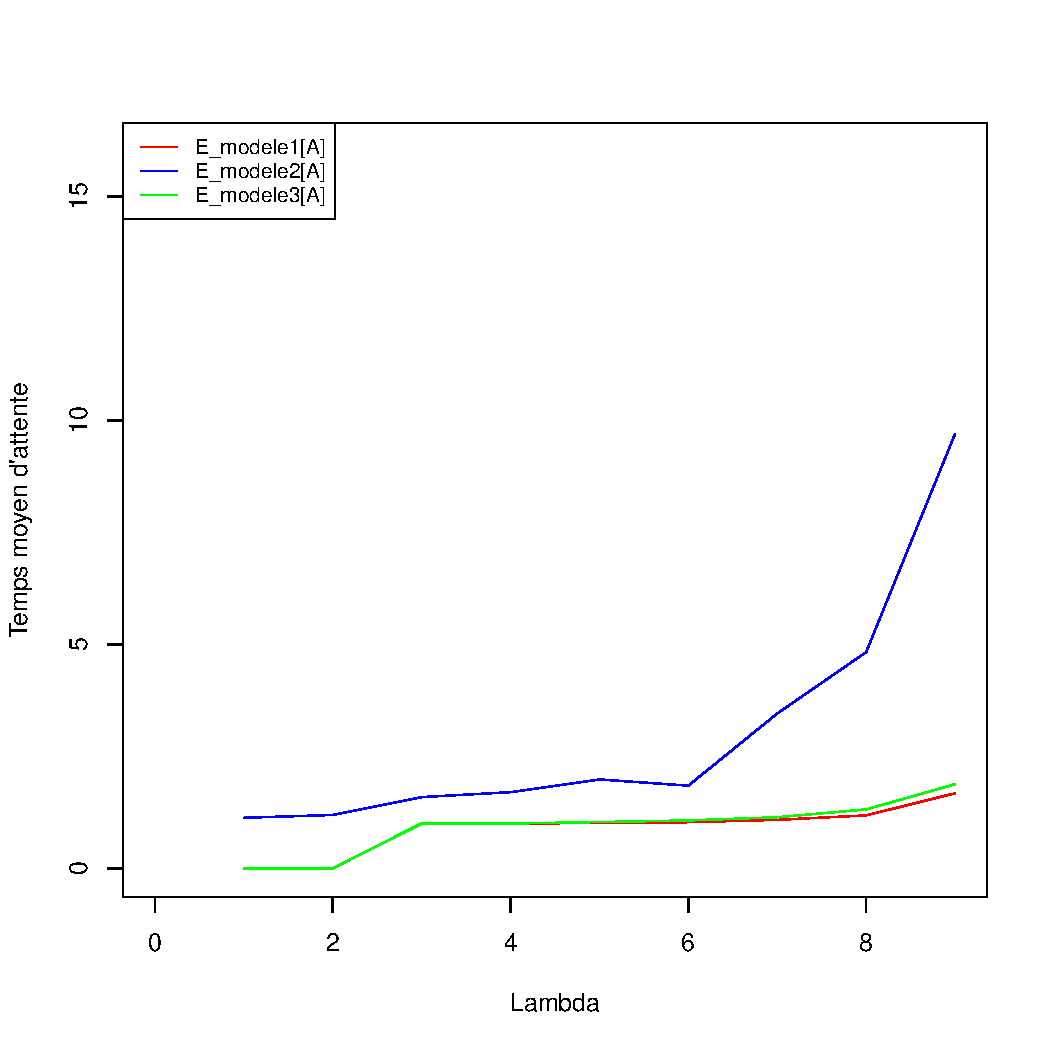
\includegraphics[scale=0.8]{E[A].pdf}}\\
	On observe que le temps moyen d'attente du modèle 2 augmente significativement à partir de lambda = 6. En effet il passe de moins de 3 à lambda = 6 à plus de 5 à lambda = 8.
	Cela s'explique par la manière dont se calcule le temps moyen d'attente dans une M/M/1. En effet on fait : \\
		$E[A] = \rho * \frac{\frac{1}{\mu}}{1-\rho}$\\
		avec : $\rho = \frac{\lambda}{\mu}$\\
		Donc plus lambda augmente, plus la valeur de rho est grande est donc plus le temps moyen d'attente est grand.
		En effet la multiplication par rho augmente plus la valeurs de E[A] que la division car rho > 1 - rho.
		A condition bien evidemment que ${\mu}$ ne soit pas trop élèvé, ce qui rendrait toute les valeurs de E[A] quasiments similaires à cause du ${\frac{1}{\mu}}$
	
	On observe que les modèles 1 et 3 ont des valeurs similaires de temps moyen d'attente. Cela s'explique par la similarité de leurs fonctionnement. En effet le modèle 1
	il y a une file avec 10 serveurs et dès qu'un serveur est libre on fais un service. Dans le 3 il y a 10 files et les clients vont dans la file la plus vide. Ainsi 
	dans les deux cas les clients sont servis dès qu'une place est libéré, que ce soit un serveur ou une file qui se libère. Cela explique bien la ressemblance des deux courbes. 
	Nous notons aussi que les temps moyen d'attente sont plus faibles pour le modèle 1 et 3 que pour le modèle 2. Cela vient du fait que le patron choisit aléatoirement un ordinateur, cela peut donc 
	de temps en temps ralentir le service car un client sera mis sur un ordinateur ou il y a déjà des clients qui attendent. Et donc cela augmentera le temps moyen d'attente de manière
	significative pour un grand nombre de clients.
	\newpage
	Le graphique des $90_{ème}$ percentiles : \\
	\label{fig2}
	\centerline{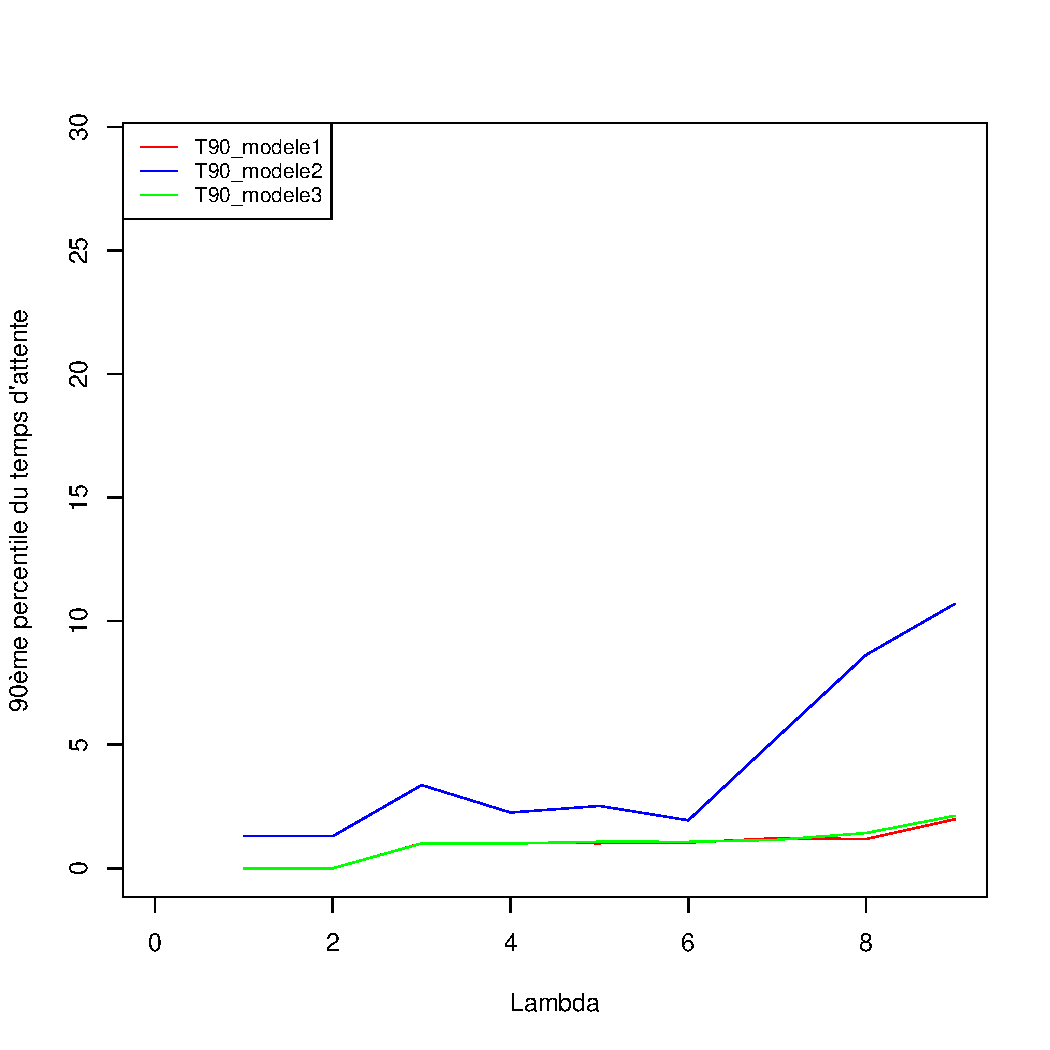
\includegraphics[scale=0.8]{t90.pdf}}\\
	
	On observe les mêmes résultats que pour le graphique précedent à l'exception de ce sursaut pour le modèle 2 à lambda = 3. 
	Cela s'explique par une "malchance" qui a fais que plusieurs clients ont été 
	mis sur des files dont le temps d'attente fût long comme expliqué au dessus, ce qui a donc augmenter le nombre de valeurs extrêmes dans le temps d'attente des clients. Or le $90_{ème}$ percentile
	prend la valeur dont 90\% des valeurs sont inférieures, donc si 10\% des valeurs des temps d'attente sont extrêmes, alors le $90_{ème}$ percentile le sera aussi.

\section{Explication des résultats théoriques}
	Les résultats théoriques que nous avons obtenu concernes uniquement les moyennes et les 90 percentiles des modèles 1 et 2.
	\subsection{moyennes théoriques}
	On constate en analysant les courbes théorique pour les temps d'attente des modèle 1 et 2 (\hyperref[fig1]{graphe 1}) que le modèle 1 est plus performant. En ce qui concerne le premier modèle la courbe est quasiment constante jusqu'a $lambda = 8$ ou elle commence à croître légèrement, le temps d'attente restant faibles.
	Pour le second modèle on constante que la courbe croît plus vite que celle du premier et dans ce graph vient a dépasser les valeurs pratiques obtenu lors de la simulation.
	\subsection{90 percentiles theoriques}
	On constate en analysant les courbes théorique pour les 90 percentile du temps d'attente des modèle 1 et 2 (\hyperref[fig2]{graphe 2}) que les courbes théoriques ont le même comportement que celles des moyenne du temps d'attente.
	Ainsi on peut voir que le modèle 1 reste le meilleur en théorie sur cette valeur.
	
\section{Conclusion}
	Après l'analyse des résultats obtenue par simulation des différents modèles, on peut conclure que les modèles les plus intéressants pour le patron du cyber café sont les modèles 1 et 3. Le modèle 1 étant le plus facile à mettre en place puisqu'il ne nécessite qu'une file pour fonctionner.
	
\section{annexe}
\label{annexe}
	\subsection{modèle 1}
		\subsubsection{Arrivee Client}
	\begin{lstlisting}
n++; 
Nentree ++; 
if(n<=N){
	event e2;
	e2.type = 1; //service
	e2.date = e.date + Exponnentielle(Mu);
	e2.etat = 0; //non traite
	Ajouter_Ech(e2);
}
temps = e.date;
	\end{lstlisting}
		\subsubsection{Service event}
	\begin{lstlisting}
if (n > 0){
	n--;

	if(n >= N){
		event e2;
		e2.type = 1; //service
		e2.date = e.date + Exponnentielle(Mu);
		e2.etat = 0;
		e2.file = -1;
		Ajouter_Ech(e2);
	}
}
	\end{lstlisting}
	\subsection{modèle2}
		\subsubsection{Arrivee Client}
			\begin{lstlisting}
double alea = (double)random()/RAND_MAX;//entre 0 et 1
if(alea < 0.1){//represente la proba que le client entre dans la file
	if(n==1){
		event e2;
		e2.type = 1; //service
		e2.date = e.date + Exponnentielle(Mu);
		e2.etat = 0; //non traite
		Ajouter_Ech(e2);
	}
	n++;
	Nentree ++;
}
temps = e.date;
			\end{lstlisting}
		\subsubsection{Service event}
			\begin{lstlisting}
if (n > 0){
	n--;
	if(n > 1){
		event e2;
		e2.type = 1; //service
		e2.date = e.date + Exponnentielle(Mu);
		e2.etat = 0;
		e2.file = -1;
		Ajouter_Ech(e2);
	}
}
			\end{lstlisting}
	\subsection{modèle3}
		\subsubsection{Arrivee Client}
			\begin{lstlisting}
int min = 0;
min = Tabmodele3[0];
int indicemin = 0;
//choix de la file avec le plus petit nombre de clients
for (int i = 0; i < 10; i++)
{
	if(min > Tabmodele3[i])
	{
		min = Tabmodele3[i];
		indicemin = i;
	}
}
Tabmodele3[indicemin]+=1;//ajout d'un client dans cette file
if(Tabmodele3[indicemin]==1){
	event e2;
	e2.type = 1; //service
	e2.date = e.date + Exponnentielle(Mu);
	e2.etat = 0; //non traite
	e2.file = indicemin;//file devant traiter le service
	Ajouter_Ech(e2);
}
n++;
Nentree ++;
temps = e.date;
			\end{lstlisting}
		\subsubsection{Service event}
			\begin{lstlisting}
if (n > 0){
	n--;
	Tabmodele3[e.file] --;//-1 client de la file concernee 
	if(Tabmodele3[e.file] > 0){
		event e2;
		e2.type = 1; //service
		e2.date = e.date + Exponnentielle(Mu);
		e2.etat = 0;
		e2.file = e.file;
		Ajouter_Ech(e2);
	}
}
temps = e.date;
			\end{lstlisting}
\end{document}
